%% TScIT template format (University of Twente Bachelor Student Conference).
\documentclass[acmtog, authorversion]{acmart}
\usepackage[htt]{hyphenat}
\usepackage{graphicx}
\graphicspath{{figures/}}
\usepackage{booktabs}
\usepackage{multirow}
\usepackage{url}
\usepackage{xcolor}
\usepackage{amssymb}
\usepackage{float}

\AtBeginDocument{%
  \providecommand\BibTeX{{%
    \normalfont B\kern-0.5em{\scshape i\kern-0.25em b}\kern-0.8em\TeX}}}

%% Conference + copyright. Set the exact TScIT edition number and date below.
\setcopyright{acmcopyright}
\copyrightyear{2026}
\acmYear{2026}
\acmConference[TScIT]{Twente Student Conference on IT}{July~2026}{Enschede, The Netherlands}
\settopmatter{printacmref=false}

\begin{document}

\title{Drone-Based Object Detection and Explanation Using Vision-Language Models}

\author{Deividas Buinevicius}
\email{d.buinevicius@student.utwente.nl}
\affiliation{%
  \institution{University of Twente}
  \streetaddress{P.O. Box 217}
  \city{Enschede}
  \postcode{7500AE}
  \country{The Netherlands}
}
\renewcommand{\shortauthors}{Buinevicius}

% -----------------------------------------------------------------------
\begin{abstract}
Autonomous drones are increasingly used in surveillance, inspection,
search-and-rescue, and environmental monitoring, where reliable object
detection is essential. Conventional detectors such as YOLO provide
bounding boxes, class labels, and confidence scores, but they do not
explain why a detection was made. This paper investigates whether
Vision-Language Models (VLMs) can support drone-based object detection
by providing both object localization and human-readable explanations.
We compare a fine-tuned YOLO11s detector with Qwen3-VL-2B-Instruct and
Gemma~4~E2B~IT on the VisDrone dataset under two evaluation settings:
a \emph{hybrid} setting in which YOLO localizes objects and the VLM
explains each detection, and a \emph{pure-VLM} setting in which the
VLM performs both localization and explanation without any detector
assistance. Detection performance is measured using standard COCO
metrics (mAP and recall), while explanation quality is assessed
using a five-criterion rubric covering visual grounding, correctness,
relevance, absence of hallucination, and usefulness.
Our results show that fine-tuned YOLO achieves mAP@0.5 of 0.298,
substantially outperforming pure-VLM approaches (Gemma~4: 0.011;
Qwen3-VL: 0.023). In the hybrid setting the VLMs produce contextually
meaningful explanations --- scoring 8.6/10 (Qwen3-VL) and 7.7/10
(Gemma~4) on a five-criterion rubric --- yet both fail to localize small, dense, or occluded objects
in the pure-VLM setting, confirming that current-generation VLMs are
better suited as an explanation layer on top of a conventional detector
than as standalone detection systems.
\end{abstract}

\keywords{Drone Vision, Object Detection, YOLO, Vision-Language Models,
Explainable AI, VisDrone}

\maketitle

% -----------------------------------------------------------------------
\section{Introduction}

Unmanned Aerial Vehicles (UAVs) are increasingly deployed in tasks
where perception is critical, including infrastructure inspection,
traffic monitoring, surveillance, and search-and-rescue operations.
Object detection is a central component of such systems, as drones
must reliably identify pedestrians, vehicles, cyclists, and other
scene elements in real time.

Traditional object detectors, including YOLO-style models, are
efficient and accurate for predefined object classes~\cite{redmon2016yolo}.
Their output is typically limited to a bounding box, a class label,
and a confidence score. These outputs indicate \emph{what} was
detected, \emph{where} it was detected, and \emph{how confident}
the model is, but they do not explain \emph{which visual evidence}
supported the prediction. In safety-critical or operator-assisted
systems, this lack of explanation increases cognitive load, since
operators must interpret and verify detections without additional
context. This can reduce trust, slow decision-making, and complicate
post-hoc failure analysis.

Recent Vision-Language Models (VLMs) can connect visual information
with natural language and may support open-vocabulary recognition and
explanation. UAV-related work such as CognitiveDrone demonstrates
that vision-language reasoning can improve cognitive drone
tasks~\cite{lykov2025cognitivedrone}, while LLVM-Drone shows that
language models can support UAV visual tasks when combined with
reliable lightweight vision models~\cite{hu2025llvmdrone}. However,
VLMs are substantially more computationally demanding than
conventional detectors: even compact models require several seconds
per inference call on a dedicated GPU, making real-time deployment on
resource-constrained drone hardware impractical with current
technology. It also remains unclear how well VLMs can localize
objects in aerial imagery and whether their explanations are actually
grounded in the image rather than being hallucinated.

This paper investigates the use of VLMs for explainable drone-based
object detection. The aim is not only to measure detection accuracy,
but also to evaluate whether the explanations produced by VLMs are
meaningful and useful for human operators. Specifically, we address
three research questions:

\begin{itemize}
  \item \textbf{RQ1:} How accurately can Qwen3-VL-2B-Instruct and
    Gemma~4~E2B~IT localize and classify objects in VisDrone images
    compared to a YOLO-style baseline, measured using IoU, precision,
    recall, and mAP?
  \item \textbf{RQ2:} To what extent are the natural-language
    explanations generated by the selected VLMs correct, visually
    grounded, and useful for interpreting object detections in drone
    imagery?
  \item \textbf{RQ3:} Under which aerial image conditions, such as
    small objects, occlusion, clutter, low resolution, or unusual
    viewpoints, do VLM-based localization and explanation outputs
    become unreliable?
\end{itemize}

The remainder of this paper is organised as follows.
Section~\ref{sec:related} reviews related work and positions this
study against it. Section~\ref{sec:background} introduces the
detection and vision-language background and defines the evaluation
metrics. Section~\ref{sec:methodology} describes the methodology and
Section~\ref{sec:setup} the experimental setup.
Section~\ref{sec:results} reports the results,
Section~\ref{sec:discussion} interprets them, and
Section~\ref{sec:conclusion} concludes.

% -----------------------------------------------------------------------
\section{Related Work}
\label{sec:related}

\subsection{Drone Imagery and Object Detection}

Drone imagery is challenging because objects are often small,
occluded, densely distributed, or viewed from unusual angles.
Datasets such as VisDrone provide aerial images with bounding box
annotations and are widely used to benchmark UAV object detection
methods~\cite{zhu2018visdrone}. Conventional detectors such as YOLO
are suitable for real-time drone perception but are limited to fixed
class lists and do not provide explanations~\cite{redmon2016yolo}.
The recurring VisDrone detection challenges document how small,
densely packed, and occluded objects remain the dominant difficulty in
this domain~\cite{cao2021visdrone}, a problem surveyed more broadly for
small-object detection~\cite{nikouei2025sod}.

\subsection{Vision-Language Models}

Vision-Language Models offer a different approach by linking image
content to natural language. CLIP introduced strong zero-shot
image-text understanding~\cite{radford2021clip}, while models such
as Grounding DINO extend this idea toward open-vocabulary object
detection~\cite{liu2023groundingdino}. SAM further supports
region-level analysis through promptable
segmentation~\cite{kirillov2023sam}. These models enable systems to
detect objects outside fixed class lists and generate natural-language
descriptions of visual content. Instruction-tuned models such as LLaVA
extended these capabilities to free-form multimodal
dialogue~\cite{liu2023llava}, and models such as Qwen2-VL added
explicit visual grounding through text-based
coordinates~\cite{wang2024qwen2vl}; however, such models are prone to
object hallucination, which motivates careful evaluation of
explanation faithfulness~\cite{li2023pope}. Their generality comes at a
cost,
however: VLMs are large transformer-based models with billions of
parameters, requiring significant GPU memory and incurring inference
latencies that are orders of magnitude higher than those of
specialized detectors such as YOLO.

\subsection{VLMs for UAV Applications}

Recent UAV research has started to integrate language reasoning into
drone systems. CognitiveDrone proposes a Vision-Language-Action model
that uses image and language input to generate drone control commands.
Its improved version adds a separate reasoning module, improving
performance on reasoning, human recognition, and symbol understanding
tasks~\cite{lykov2025cognitivedrone}. LLVM-Drone combines large
language models with lightweight vision models including YOLO, SAM,
RAM, and Grounded SAM. The authors emphasize that large multimodal
models can hallucinate and that specialized vision models remain
important for reliable perception~\cite{hu2025llvmdrone}.

Existing UAV-related VLM research primarily focuses on high-level
reasoning or combines language models with separate vision modules,
rather than directly evaluating whether VLMs can both localize objects
and explain their predictions in aerial imagery. This gap motivates
the present work. Table~\ref{tab:positioning} positions this study
against representative prior work.

\begin{table}[H]
\caption{Positioning of this work against representative prior work.
  \textbf{Aerial} = evaluated on aerial/UAV imagery;
  \textbf{VLM} = uses a vision-language model;
  \textbf{Loc.} = evaluates object localization quantitatively;
  \textbf{Expl.} = evaluates natural-language explanation quality;
  \textbf{Hybrid} = combines a conventional detector with a VLM.}
\label{tab:positioning}
\resizebox{\columnwidth}{!}{%
\begin{tabular}{lccccc}
\toprule
Study & Aerial & VLM & Loc. & Expl. & Hybrid \\
\midrule
YOLO~\cite{redmon2016yolo}                    & --         & --         & \checkmark & --         & -- \\
CLIP~\cite{radford2021clip}                   & --         & \checkmark & --         & --         & -- \\
Grounding DINO~\cite{liu2023groundingdino}    & --         & \checkmark & \checkmark & --         & -- \\
CognitiveDrone~\cite{lykov2025cognitivedrone} & \checkmark & \checkmark & --         & --         & -- \\
LLVM-Drone~\cite{hu2025llvmdrone}             & \checkmark & \checkmark & \checkmark & --         & \checkmark \\
VisDrone-DET2021~\cite{cao2021visdrone}       & \checkmark & --         & \checkmark & --         & -- \\
Small-object survey~\cite{nikouei2025sod}     & \checkmark & --         & \checkmark & --         & -- \\
LLaVA~\cite{liu2023llava}                     & --         & \checkmark & --         & --         & -- \\
POPE~\cite{li2023pope}                        & --         & \checkmark & --         & \checkmark & -- \\
\midrule
\textbf{This work}                            & \checkmark & \checkmark & \checkmark & \checkmark & \checkmark \\
\bottomrule
\end{tabular}}
\end{table}

% -----------------------------------------------------------------------
\section{Background}
\label{sec:background}

\subsection{Object Detection and YOLO}
Single-stage detectors predict object locations and classes in one
forward pass, trading some accuracy for the speed required by
real-time applications. The YOLO family popularised this paradigm by
framing detection as direct bounding-box and class regression over an
image grid~\cite{redmon2016yolo}. This study uses YOLO11, a recent
Ultralytics iteration with an anchor-free detection head, as its
baseline detector~\cite{jocher2024yolo11}. Such detectors are fast and
accurate on their trained classes but are restricted to a fixed label
set and emit no explanation of their predictions. Aerial imagery is
particularly demanding: objects are frequently very small, densely
packed, and heavily occluded, which the VisDrone detection
challenges identify as the dominant source of
difficulty~\cite{cao2021visdrone} and which recent small-object
detection surveys analyse in depth~\cite{nikouei2025sod}.

\subsection{Vision-Language Models}
Vision-Language Models couple a visual encoder with a language model
through a projection module and are driven by natural-language
prompts. Instruction tuning on image--text pairs produced
general-purpose multimodal assistants such as LLaVA that follow
free-form visual instructions~\cite{liu2023llava}. More recent models
additionally emit \emph{grounded} outputs: Qwen2-VL and Qwen3-VL are
trained to return object coordinates as text and to process images at
native, variable resolution~\cite{wang2024qwen2vl, bai2025qwen3vl},
while the Gemma line provides compact open multimodal models intended
for resource-constrained hardware~\cite{gemmateam2025gemma3,
google2026gemma4}. Because these models produce coordinates through
language modelling rather than a dedicated detection head, their
localization behaviour differs fundamentally from YOLO --- a contrast
this study examines directly. A well-documented failure mode is object
hallucination, in which a VLM describes objects that are not present
in the image~\cite{li2023pope}.

\subsection{Detection Evaluation Metrics}
Detection quality is measured with the standard COCO metrics, all
built on the Intersection-over-Union (IoU) between a predicted box
$B_p$ and a ground-truth box $B_{gt}$:
\begin{equation}
\mathrm{IoU}(B_p, B_{gt}) = \frac{|B_p \cap B_{gt}|}{|B_p \cup B_{gt}|}.
\end{equation}
A prediction is a true positive when its IoU with a same-class
ground-truth box exceeds a threshold $\tau$. Precision is the fraction
of predictions that are correct and recall the fraction of
ground-truth objects retrieved:
\begin{equation}
P = \frac{TP}{TP + FP}, \qquad R = \frac{TP}{TP + FN}.
\end{equation}
Average Precision (AP) is the area under the precision--recall curve
for a class, and mean Average Precision (mAP) averages AP over all
classes. We report mAP@0.5 ($\tau = 0.5$), mAP@0.75 ($\tau = 0.75$),
and mAP@0.5:0.95 (averaged over $\tau \in \{0.50, 0.55, \dots, 0.95\}$)
following the COCO protocol, together with per-class AP and the
size-stratified scores mAP$_{\text{small}}$, mAP$_{\text{medium}}$,
and mAP$_{\text{large}}$. All metrics are computed with
\texttt{pycocotools} after converting predictions and annotations to
COCO format.

% -----------------------------------------------------------------------
\section{Methodology}
\label{sec:methodology}

\subsection{Dataset}

We use the VisDrone-DET dataset~\cite{zhu2018visdrone}, which contains
real aerial drone imagery annotated with bounding boxes across ten
object classes: \emph{pedestrian}, \emph{people}, \emph{bicycle},
\emph{car}, \emph{van}, \emph{truck}, \emph{tricycle},
\emph{awning-tricycle}, \emph{bus}, and \emph{motor}. All experiments
use the official validation split of 548 images. Annotations are
converted to COCO format for compatibility with standard evaluation
tooling.

\begin{figure}[htbp]
  \centering
  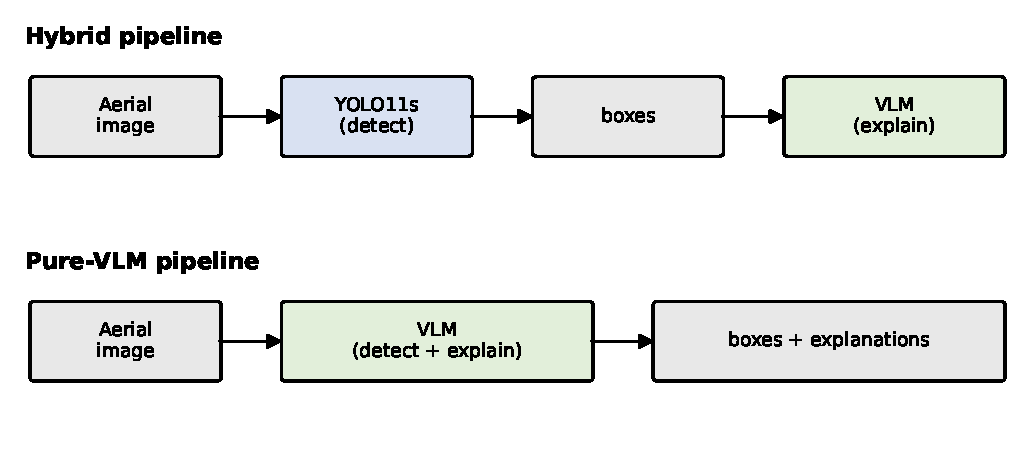
\includegraphics[width=\columnwidth]{figures/system_overview.pdf}
  \caption{The two evaluation settings. In the hybrid setting YOLO11s
    detects objects and the VLM explains each box; in the pure-VLM
    setting the VLM both detects and explains.}
  \label{fig:overview}
\end{figure}

\subsection{YOLO Baseline}

We evaluate two YOLO configurations as baselines:

\begin{itemize}
  \item \textbf{YOLO11n pretrained on COCO} --- a lightweight model
    with 80 generic classes. Class names are mapped to VisDrone
    equivalents where possible (e.g., \textit{person} $\to$
    \textit{pedestrian}).
  \item \textbf{YOLO11s fine-tuned on VisDrone} --- YOLO11s fine-tuned
    on the VisDrone training split; this serves as the primary YOLO
    baseline. The training procedure is detailed in
    Section~\ref{sec:yolotrain}.
\end{itemize}

Detection performance is evaluated using pycocotools with standard
COCO metrics: mAP@0.5, mAP@0.5:0.95, mAP@0.75, and recall, as well as
per-class AP.

\subsection{Fine-Tuning the YOLO Baseline}
\label{sec:yolotrain}

The primary detector is obtained by fine-tuning YOLO11s on VisDrone
rather than training from scratch. We start from the COCO-pretrained
\texttt{yolo11s.pt} checkpoint and continue training on the
VisDrone~2019-DET training split, using a YOLO-format version of the
dataset whose labels cover the same ten object classes used throughout
this study (the VisDrone \emph{ignored-region} and \emph{others}
categories are excluded). Transfer learning from COCO lets the model
reuse general low-level visual features and adapt only to the aerial
domain and the VisDrone label set.

Training uses the Ultralytics framework on a single Kaggle T4 GPU with
the following configuration: 50 epochs at an input resolution of
$640\times640$, batch size 16, and a cosine learning-rate schedule.
Early stopping is applied with a patience of 15 epochs, so training
halts if validation performance does not improve for 15 consecutive
epochs. Mosaic augmentation is enabled during training and disabled for
the final 10 epochs, allowing the model to converge on undistorted
images; all remaining hyperparameters (optimizer, base learning rate,
and the other augmentations) are left at the Ultralytics defaults. The
checkpoint with the best validation score is retained as the final
model.

This fine-tuned model serves both as the standalone detection baseline
(RQ1) and as the localizer in the hybrid pipeline, where it supplies the
boxes that the VLMs explain. On the 548-image validation split it
reaches an mAP@0.5 of 0.298 (Table~\ref{tab:overall}), far above the
COCO-pretrained YOLO11n and the pure-VLM models, establishing the upper
reference point against which VLM localization is measured.

\subsection{VLM Models}

The VLM-based part of the study uses two models evaluated in
inference-only mode without fine-tuning. Lightweight 2-billion
parameter variants were chosen deliberately: real drone hardware
has strict size, weight, and power constraints that make deploying
large models impractical, so evaluating compact models reflects the
conditions under which such a system would realistically operate.
In half precision (fp16) both models fit comfortably within the
memory budget of a Kaggle T4 GPU (15~GB VRAM) --- each occupies
roughly 5~GB --- which is the compute environment used for all
experiments; no quantization was required.

\begin{itemize}
  \item \textbf{Qwen3-VL-2B-Instruct} --- selected for its explicit
    support of spatial visual understanding including object positions,
    viewpoints, occlusions, and grounding~\cite{bai2025qwen3vl,
    wang2024qwen2vl}. It uses a dynamic resolution
    patching system that preserves fine-grained detail in high-resolution
    aerial images.
  \item \textbf{Gemma~4~E2B~IT} --- the \texttt{google/gemma-4-E2B-it}
    checkpoint, a compact open multimodal model intended for efficient
    on-device deployment~\cite{google2026gemma4}, which makes it a
    realistic lightweight counterpart to Qwen3-VL under the same hardware
    constraints.\footnote{The \texttt{E2B} suffix denotes the model's
    \emph{effective} ($\approx$2B) parameter count, an elastic-parameter
    naming convention first introduced in the Gemma~3n line and carried
    into this release; it does not indicate a Gemma~3n model. We report
    results for exactly the \texttt{google/gemma-4-E2B-it} checkpoint as
    documented by Google~\cite{google2026gemma4} (accessed June~2026); at
    the time of writing no peer-reviewed technical report for this
    specific model was available, so we cite the official model
    documentation.}
\end{itemize}

VLM inference is nevertheless far slower than a conventional
detector: in the pure-VLM setting a single full-image detection call
averages about 38~seconds, so processing the full 548-image
validation set requires roughly six hours of continuous GPU time per
model. This stands in sharp contrast to YOLO11s, which
processes the entire validation set in under one minute. The
pure-VLM setting evaluates the full 548-image validation split;
due to this inference cost the hybrid explanation setting evaluates
a curated 30-image sample selected to cover diverse scene
difficulties (Section~\ref{sec:rq2sample}).

\subsection{Evaluation Settings}

Two inference settings are evaluated:

\textbf{Hybrid setting.} The fine-tuned YOLO11s first runs on each
image and produces bounding box detections. For each detection the VLM
receives the original image with the detected bounding box highlighted
in red and is prompted to generate a single natural-language explanation
describing the visual evidence that supports the detection. This setting
isolates explanation quality from localization accuracy.

\textbf{Pure-VLM setting.} The VLM receives the raw aerial image
without any detector assistance and is asked to identify all visible
objects from the VisDrone class list, outputting bounding box
coordinates along with a brief explanation for each detection. This
setting evaluates whether VLMs can serve as standalone
detection-and-explanation systems.

\subsection{RQ2 Evaluation Sample}
\label{sec:rq2sample}

Explanation quality (RQ2) is evaluated on a curated 30-image sample
drawn from the VisDrone validation set. Images are stratified into
five scene types to ensure coverage of diverse conditions:
core mixed-difficulty, easy single-class, hard dense/occluded,
high-resolution, and sparse scenes. These RQ2 scene types are a
separate stratification from the RQ3 difficulty groups
(Section~\ref{sec:results}), which are labelled A--E; the two
groupings should not be conflated. This sample is used for both VLMs in
the hybrid setting.

\subsection{Explanation Quality Rubric}

To address RQ2, a sample of VLM-generated explanations is manually
scored using a five-criterion rubric, each criterion scored 0--2
for a maximum of 10 points per explanation:

\begin{enumerate}
  \item \textbf{Visual grounding} --- does the explanation reference
    specific visible features such as shape, shadow, colour, or
    position?
  \item \textbf{Correctness} --- is the description accurate for the
    detected object?
  \item \textbf{Relevance} --- is the explanation focused on the
    detected object rather than background or other objects?
  \item \textbf{No hallucination} --- does the explanation avoid
    invented details not visible in the image?
  \item \textbf{Usefulness} --- would the explanation help a human
    operator understand or verify the detection?
\end{enumerate}

\subsection{Justification of Design Choices}
Each component was chosen to reflect a realistic, resource-constrained
drone deployment. \textbf{YOLO11s} is the primary baseline because it
is a current, lightweight single-stage detector that runs in real time
on modest hardware, and fine-tuning it on VisDrone provides a strong
domain-specific reference. \textbf{Qwen3-VL-2B} and \textbf{Gemma~4~E2B}
were selected as the two VLMs because both are compact, openly
available, instruction-tuned multimodal models that fit a single T4
GPU, with complementary design emphases --- Qwen3-VL on explicit
spatial grounding, Gemma~4 on efficient on-device multimodality ---
making them a meaningful contrast under the same constraints.
\textbf{VisDrone} is used because it is a standard aerial-detection
benchmark and exposes the small, dense, and occluded objects central to
RQ3. The \textbf{hybrid and pure-VLM split} isolates the two questions:
the pure setting tests whether a VLM can localise (RQ1), while the
hybrid setting removes localisation from the VLM so that explanation
quality (RQ2) can be judged independently of detection accuracy. The
\textbf{30-image RQ2 sample} and \textbf{25-image RQ3 set} are
hand-stratified across difficulty conditions because both require
manual, per-detection judgement that does not scale to all 548 images.
Finally, a \textbf{manual rubric} rather than an automated text-overlap
metric such as BLEU is used for RQ2 because there is no reference
explanation to match against, and the qualities of interest --- visual
grounding and hallucination --- cannot be captured by $n$-gram overlap.

\subsection{Statistical Analysis}
Detection metrics (RQ1) are reported as point estimates computed with
\texttt{pycocotools} over the full 548-image validation set. For the
explanation rubric (RQ2), each criterion is summarised by its mean
score across the $n = 90$ scored explanations per model (the top three
detections per image over the 30-image sample). The two models are
compared per criterion, and their per-explanation totals are compared
with a paired Wilcoxon signed-rank test over the detections scored for
both models.

% -----------------------------------------------------------------------
\section{Experimental Setup}
\label{sec:setup}

\subsection{Compute Environment}
All experiments run in a Kaggle notebook with a single NVIDIA Tesla~T4
GPU (15~GB VRAM). YOLO11s is fine-tuned for 50 epochs at
$640\times640$ input resolution. Both VLMs run in half precision
(fp16) without quantization; each occupies roughly 5~GB, well within
the T4 budget.

\subsection{Models and Inference Configuration}
The VLMs are the pinned checkpoints \texttt{Qwen/Qwen3-VL-2B-Instruct}
and \texttt{google/gemma-4-E2B-it}, loaded through the Hugging Face
\texttt{transformers} library with the SDPA attention backend.
Decoding is greedy (\texttt{do\_sample = False}) in every setting. In
the hybrid setting the highlighted image is down-scaled to a long side
of 1280~px and the explanation is capped at 64 new tokens. In the
pure-VLM setting the image is capped at $1280\times1280$~px and
generation at up to 1536 new tokens (detection) or 2048 (detection
plus explanation). The exact prompts are reproduced in
Appendix~\ref{app:prompts}.

\subsection{Pipeline and Recorded Outputs}
In the hybrid pipeline, YOLO11s detects objects (confidence threshold
0.40) and the VLM then explains each retained box in turn. In the
pure-VLM pipeline, the VLM is queried once per image and its JSON
output is parsed into detections. Each model is decoded with a
\emph{separate} parser matched to its own coordinate convention
(Qwen3-VL \texttt{[x1,y1,x2,y2]}, Gemma~4 the Gemini-style
\texttt{[y1,x1,y2,x2]}; Appendix~\ref{app:prompts}); coordinates are
returned in a $0$--$1000$ normalised space and rescaled to pixels. We
validated this decoding per model: across all 548 images, every one of
the 19{,}587 Qwen3-VL and 7{,}423 Gemma~4 predicted boxes satisfies
$x_1 < x_2$ and $y_1 < y_2$ and lies within the image bounds (zero
violations of either condition). This confirms that no coordinate-order
transposition occurs and that the low pure-VLM mAP reflects genuine
under-detection and loose localisation rather than a parsing artifact.
For every image
the pipeline records the detections (class, box, confidence), the
explanation text, and the per-call latency, and checkpoints results to
JSON so that long runs can be resumed.

\subsection{Reproducibility}
All experiments were run in a Kaggle notebook with a single NVIDIA
Tesla~T4 GPU. The VLMs are the pinned Hugging Face checkpoints
\texttt{Qwen/Qwen3-VL-2B-Instruct} and \texttt{google/gemma-4-E2B-it},
loaded with the \texttt{transformers} library in half precision and
without quantization; YOLO11s was fine-tuned with the Ultralytics
library. The five pipeline notebooks, the evaluation scripts, and the
generated prediction and explanation files are available in the project
repository.

% -----------------------------------------------------------------------
\section{Results}
\label{sec:results}

\subsection{Detection Performance (RQ1)}

Table~\ref{tab:overall} shows overall detection metrics across all
evaluated models on the VisDrone validation set (548 images).
The fine-tuned YOLO11s achieves the highest mAP@0.5 of 0.298,
substantially outperforming all other configurations. The
COCO-pretrained YOLO11n achieves mAP@0.5 of 0.053, limited by
class mapping mismatches and the domain gap between COCO and
aerial imagery. Both VLMs in the pure-VLM setting achieve very
low mAP@0.5 (Gemma~4: 0.011; Qwen3-VL: 0.023), reflecting
fundamental difficulties in producing well-calibrated bounding
boxes from language-model inference alone; Qwen3-VL roughly doubles
Gemma~4's detection accuracy but both remain an order of magnitude
below the fine-tuned YOLO11s.

\begin{table}[H]
\caption{Overall detection metrics on VisDrone validation set (548 images).
  R = Recall@0.5. Precision@0.5 is omitted: under the COCO definition it is the
  area under the precision--recall curve, which equals AP@0.5 (the mAP@.5
  column), so it carries no additional information. The hybrid setting is
  omitted: detection is performed by YOLO11s, so its metrics are identical to
  the YOLO11s row.}
\label{tab:overall}
\resizebox{\columnwidth}{!}{%
\begin{tabular}{lrrrr}
\toprule
Model & mAP@.5 & mAP@.5:.95 & mAP@.75 & R \\
\midrule
YOLO11n          & 0.053 & 0.036 & 0.039 & 0.067 \\
YOLO11s-tuned    & 0.298 & 0.188 & 0.198 & 0.357 \\
Gemma~4~E2B      & 0.011 & 0.004 & 0.002 & 0.030 \\
Qwen3-VL-2B      & 0.023 & 0.015 & 0.015 & 0.056 \\
\bottomrule
\end{tabular}}
\end{table}

Across object size bands (Table~\ref{tab:size}), both YOLO
configurations drop sharply on small objects, consistent with the
well-known difficulty of small-object detection in aerial imagery, but
the VLMs collapse almost entirely: Gemma~4 scores effectively zero and
Qwen3-VL only 0.005 mAP\textsubscript{small}, indicating that without a
detection head small objects are rarely localised at all.

\begin{table}[H]
\caption{Size-stratified detection mAP@0.5:0.95 on the VisDrone
  validation set (548 images).}
\label{tab:size}
\begin{tabular}{lrrr}
\toprule
Model & mAP$_{\text{small}}$ & mAP$_{\text{medium}}$ & mAP$_{\text{large}}$ \\
\midrule
YOLO11n & 0.007 & 0.054 & 0.242 \\
YOLO11s-tuned & 0.094 & 0.299 & 0.447 \\
Gemma~4~E2B & 0.000 & 0.003 & 0.077 \\
Qwen3-VL-2B & 0.005 & 0.031 & 0.200 \\
\bottomrule
\end{tabular}
\end{table}

Table~\ref{tab:perclass} reports per-class AP at IoU 0.5:0.95.
The fine-tuned YOLO11s achieves the highest per-class scores across
all categories, with car (0.513) and bus (0.328) scoring highest.
VLMs achieve their best relative performance on large, visually
distinctive vehicles (car, truck, van) and near-zero scores on small
or ambiguous classes (awning-tricycle, tricycle, bicycle).

\begin{table}[H]
\caption{Per-class AP at IoU 0.5:0.95 on the VisDrone validation set.
  G4 = Gemma~4~E2B pure VLM; Q3 = Qwen3-VL-2B pure VLM;
  YN = YOLO11n COCO pretrained; YS = YOLO11s VisDrone fine-tuned.}
\label{tab:perclass}
\begin{tabular}{lrrrr}
\toprule
Class            & G4     & Q3     & YN     & YS     \\
\midrule
pedestrian       & 0.002  & 0.006  & 0.032  & 0.159  \\
people           & 0.003  & 0.004  & 0.000  & 0.081  \\
bicycle          & 0.000  & 0.004  & 0.009  & 0.040  \\
car              & 0.013  & 0.041  & 0.185  & 0.513  \\
van              & 0.005  & 0.021  & 0.000  & 0.247  \\
truck            & 0.008  & 0.040  & 0.037  & 0.204  \\
tricycle         & 0.001  & 0.002  & 0.000  & 0.105  \\
awning-tricycle  & 0.000  & 0.000  & 0.000  & 0.054  \\
bus              & 0.005  & 0.020  & 0.090  & 0.328  \\
motor            & 0.001  & 0.010  & 0.009  & 0.154  \\
\midrule
\textbf{mean}    & \textbf{0.004} & \textbf{0.015} & \textbf{0.036} & \textbf{0.188} \\
\bottomrule
\end{tabular}
\end{table}

\begin{figure}[htbp]
  \centering
  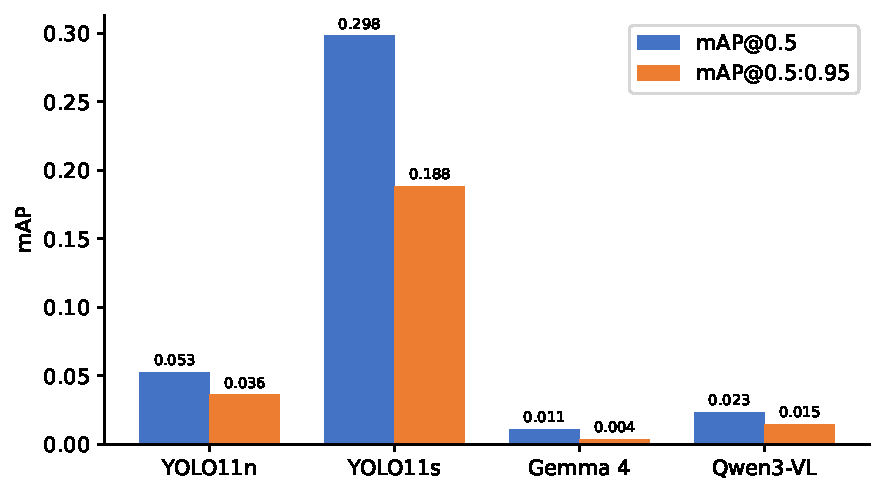
\includegraphics[width=\columnwidth]{figures/map_barchart.pdf}
  \caption{Detection mAP@0.5 and mAP@0.5:0.95 across the four models
    (visual summary of Table~\ref{tab:overall}).}
  \label{fig:map}
\end{figure}

\begin{figure}[htbp]
  \centering
  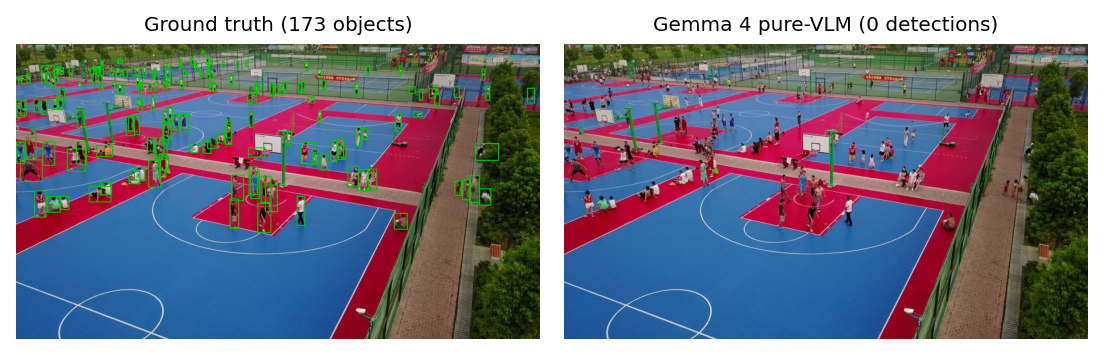
\includegraphics[width=\columnwidth]{figures/rq1_dense_comparison.png}
  \caption{Under-detection on a dense aerial scene. Left: ground-truth
    objects (green). Right: Gemma~4 pure-VLM detections (red). The VLM
    recovers only a small fraction of the objects present.}
  \label{fig:dense}
\end{figure}

\subsection{Explanation Quality (RQ2)}

We manually scored the top three highest-confidence detections per
image across the 30-image RQ2 sample for both models in the hybrid
setting (90 explanations per model) using the five-criterion rubric of
Section~\ref{sec:methodology} (each criterion 0--2; maximum 10).
Table~\ref{tab:rq2} reports the mean score per criterion.

\begin{table}[H]
\caption{Mean explanation-quality scores in the hybrid setting
  (90 explanations per model; each criterion 0--2, maximum 10).}
\label{tab:rq2}
\begin{tabular}{lrr}
\toprule
Criterion         & Qwen3-VL & Gemma~4 \\
\midrule
Visual grounding  & 1.90 & 1.80 \\
Correctness       & 1.56 & 1.46 \\
Relevance         & 1.79 & 1.39 \\
No hallucination  & 1.80 & 1.76 \\
Usefulness        & 1.60 & 1.29 \\
\midrule
\textbf{Mean total (/10)} & \textbf{8.64} & \textbf{7.69} \\
\bottomrule
\end{tabular}
\end{table}

Qwen3-VL scores higher than Gemma~4 on every criterion, with an overall
mean of 8.64/10 versus 7.69/10. Both models score highest on visual
grounding (1.90 and 1.80), indicating that their explanations typically
reference genuinely visible features rather than generic descriptions.
Contrary to our initial expectation, no-hallucination is among the
\emph{strongest} criteria for both models (1.80 and 1.76), not the
weakest: in the hybrid setting the highlighted red box anchors the VLM
to a concrete region, which appears to suppress invented detail. The
weakest criteria are correctness for Qwen3-VL (1.56) and usefulness
(1.29) and relevance (1.39) for Gemma~4, whose explanations more often
remain vague or drift to surrounding context. The largest Qwen3-VL
advantage is on relevance (1.79 vs.\ 1.39) and usefulness (1.60 vs.\
1.29). Across scene types Qwen3-VL is stable (mean totals
8.3--9.0), whereas Gemma~4 is more variable (6.5--8.5), scoring lowest
on the high-resolution group. A paired Wilcoxon signed-rank test over
the 86 detections scored for both models confirms that Qwen3-VL's
explanations are rated significantly higher than Gemma~4's
($W = 553.5$, $p = 0.001$).

\begin{figure}[htbp]
  \centering
  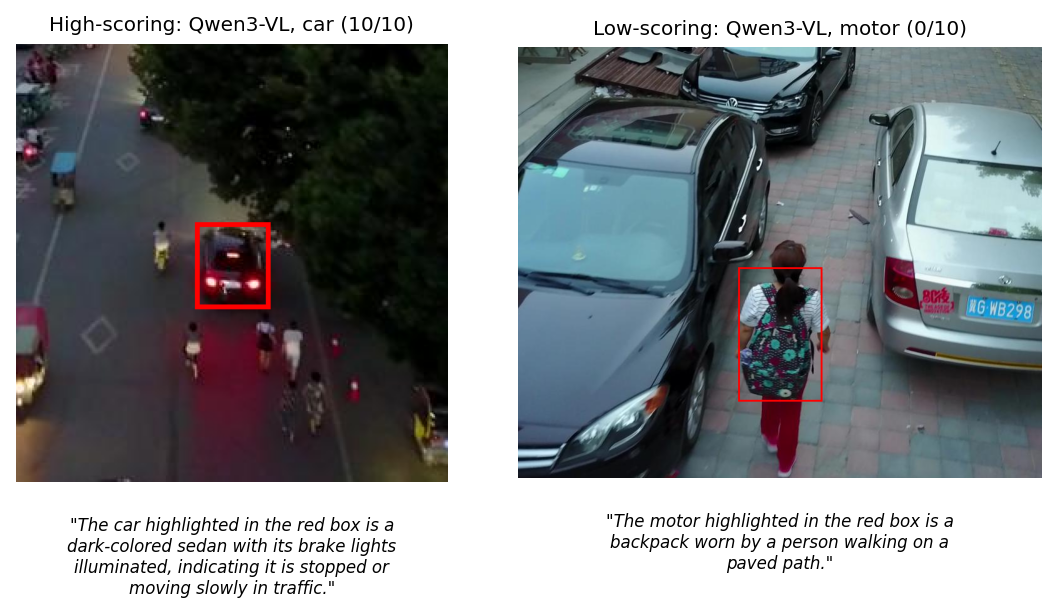
\includegraphics[width=\columnwidth]{figures/rq2_examples.png}
  \caption{Example explanations. Left: a high-scoring, visually grounded
    description of a clearly visible car. Right: a low-scoring case where
    the VLM misidentifies the highlighted object and invents details.}
  \label{fig:rq2ex}
\end{figure}

\subsection{Failure Analysis (RQ3)}

We evaluated both pure-VLM models against ground truth on a curated set
of 25 VisDrone images (five per group): (A)~tiny, dense, low-resolution
scenes, (B)~occlusion-dominant scenes, (C)~extreme object density,
(D)~mid-difficulty/high-contrast scenes, and (E)~sparse scenes (a
false-positive probe). For each image we recorded each model's
detection count against the ground-truth object count and manually
coded the dominant failure mode. Table~\ref{tab:rq3} reports the
detection ratios per group.

\begin{table}[H]
\caption{Pure-VLM detections vs.\ ground truth on the 25-image RQ3 set
  (mean over 5 images per group). Ratio = detections / ground-truth
  objects; lower means more severe under-detection.}
\label{tab:rq3}
\begin{tabular}{llrrrr}
\toprule
      &                          & \multicolumn{2}{c}{Gemma~4} & \multicolumn{2}{c}{Qwen3-VL} \\
Group & Condition (mean GT)      & ratio & dets & ratio & dets \\
\midrule
A & tiny/dense/low-res (111) &   4\% &  4.6 &  38\% & 42.4 \\
B & occlusion (45)           &  21\% &  9.4 &  83\% & 37.2 \\
C & extreme density (114)    &  17\% & 19.2 &  37\% & 42.6 \\
D & mid-difficulty (33)      &  26\% &  8.6 &  72\% & 24.0 \\
E & sparse (2)               & 100\% &  1.8 &  89\% &  1.6 \\
\bottomrule
\end{tabular}
\end{table}

Three findings stand out. First, \textbf{both models degrade sharply
with object density and small scale}: groups A and C, whose
ground-truth counts exceed 110 objects, give the lowest ratios for both
models, while the sparse group E (2 objects) is handled almost
perfectly. Second, \textbf{Qwen3-VL recovers far more objects than
Gemma~4} (group ratios 37--89\% vs.\ 4--26\%); Gemma~4 is strongly
under-detecting, reporting as few as 4\% of the objects present in the
densest scenes. Third, this higher recall has a cost: across the 25
images Qwen3-VL's dominant coded failures are \emph{under-detection}
(8 images) and \emph{hallucinated objects} (8), whereas Gemma~4's are
\emph{imprecise localization} (10) and \emph{under-detection} (8), with
only one hallucinated-object case. Gemma~4 is thus conservative --- it
misses objects and places loose boxes --- while Qwen3-VL is aggressive,
detecting more but inventing more spurious objects. In the genuinely
sparse group E both models were coded \emph{acceptable} on almost every
image, indicating that false-positive hallucination is triggered mainly
by clutter rather than emitted unconditionally.

\textbf{Imprecise localization.} Even when an object is found, the box
is approximated from visual reasoning rather than a learned detection
head, producing loose boxes; this is reflected in the collapse from
mAP@0.5 to mAP@0.75 for both models (Table~\ref{tab:overall}).

\textbf{No usable confidence.} Neither VLM emits a meaningful confidence
score, so the pipeline assigns a constant value of 1.0; confidence
thresholding is therefore unavailable as a quality filter. Because every
detection shares the same confidence, the precision--recall ranking that
average precision integrates over is governed by the model's output order
rather than by calibrated certainty, so the reported VLM mAP is partly an
artifact of detection ordering.

\begin{figure}[htbp]
  \centering
  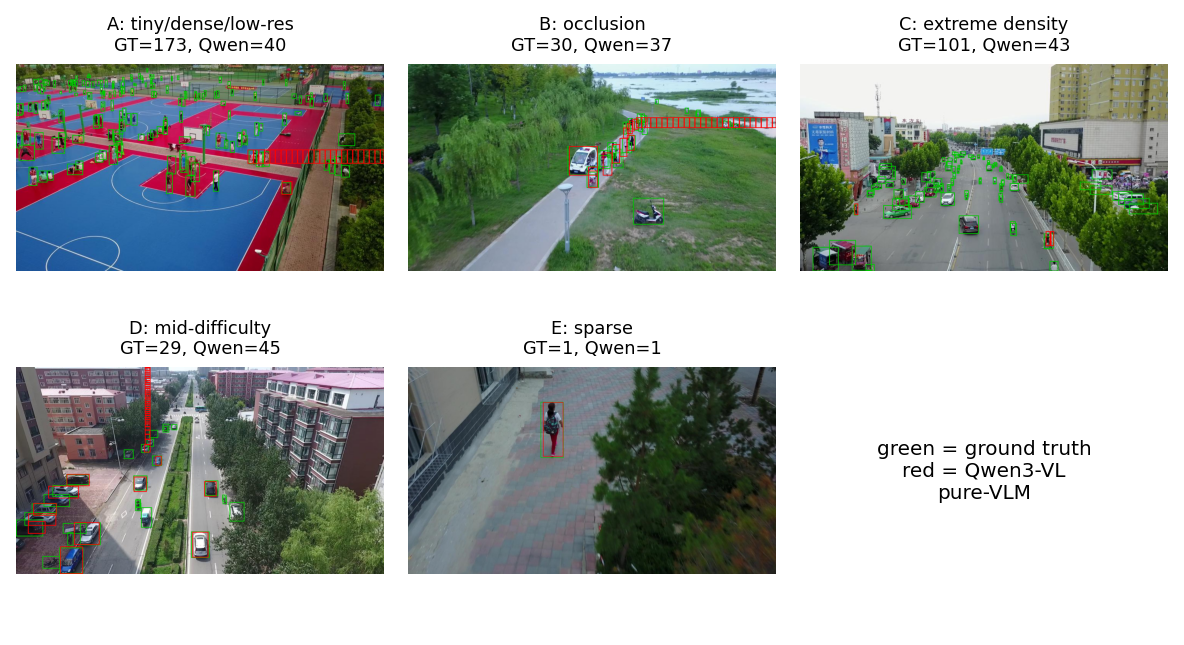
\includegraphics[width=\columnwidth]{figures/rq3_panels.png}
  \caption{One representative image per RQ3 difficulty group with
    ground-truth objects (green) and Qwen3-VL pure-VLM detections (red).
    Under-detection scales with object density (groups A and C); the
    sparse group E is handled correctly.}
  \label{fig:rq3panels}
\end{figure}

These failure modes are consistent with the observation in
LLVM-Drone~\cite{hu2025llvmdrone} that large multimodal models
can hallucinate and that specialized vision models remain important
for reliable perception in UAV systems.

% -----------------------------------------------------------------------
\section{Discussion}
\label{sec:discussion}

Across both settings, the results are best understood through a single
explanatory account, which we term the \emph{missing detection-head}
effect: a VLM approximates object locations through language-level
spatial reasoning over a fixed visual-token budget, rather than
through a dense, learned detection head. This account predicts the
three patterns examined below --- severe under-detection in crowded
scenes, loose boxes that collapse at higher IoU thresholds, and a
steep drop on small objects --- and explains why the hybrid setting,
which removes localization from the VLM's responsibilities, is the
more reliable use of the same model.

\subsection{RQ1 --- Localization Accuracy}

The results clearly show that fine-tuned YOLO11s dominates on all
detection metrics, with an mAP@0.5 of 0.298 compared to 0.011--0.023
for pure-VLM approaches. This gap is explained by several structural
differences. First, YOLO uses a learned detection head that produces
calibrated bounding boxes at pixel precision; VLMs approximate
positions through language-level spatial reasoning, producing loose
boxes. Second, the fine-tuned YOLO benefits from VisDrone-specific
training; VLMs receive no domain-specific training in this study.
Third, VLMs are not architecturally optimized for exhaustive detection
and tend to under-report objects in dense scenes. Fourth, and
practically important, VLMs are far slower: a single full-image
pure-VLM call averages roughly 38~seconds versus milliseconds for
YOLO, ruling out real-time use on current drone hardware entirely.

The COCO-pretrained YOLO11n (mAP@0.5 = 0.053) provides a useful
intermediate reference: it outperforms VLMs significantly despite
having no VisDrone training, confirming that the VLM gap is not
purely a domain-adaptation issue but reflects a fundamental
limitation in localization capability.

Qwen3-VL clearly outperforms Gemma~4 on detection (mAP@0.5 0.023 vs.\
0.011, and 0.015 vs.\ 0.004 at mAP@0.5:0.95), roughly doubling its
accuracy, though both remain far below the fine-tuned YOLO11s.
Both models perform best on large, visually salient vehicles (car,
truck, van) and worst on small objects (awning-tricycle, tricycle,
bicycle), which is consistent with the hypothesis that VLM
localization degrades with object size.

\subsection{RQ2 --- Explanation Quality}

The rubric scores confirm that the hybrid setting produces reliable
explanations overall: both models average above 7.5/10, and their
highest scores are on visual grounding, consistent with the
expectation that anchoring the VLM to a YOLO-highlighted region keeps
it tied to visible evidence. The expectation that no-hallucination
would be the weakest criterion did \emph{not} hold --- it is among the
strongest for both models, suggesting that hallucination is far less of
a problem when the VLM explains a pre-localised box than when it must
reason over a full scene (as in the pure-VLM setting). The clearest
difference between the models is qualitative: Qwen3-VL's explanations
are more relevant and useful (1.79 and 1.60) than Gemma~4's (1.39 and
1.29), which more often describe surrounding context or add little
actionable detail. This makes Qwen3-VL the more suitable explanation
layer of the two, although both are usable.

\subsection{RQ3 --- Failure Modes}

The failure analysis shows that the two VLMs fail in different ways,
revealing a recall--precision trade-off. Gemma~4 is conservative: its
dominant failures are under-detection and imprecise box placement, so
it misses most objects in dense scenes and localises loosely the ones
it does find. Qwen3-VL is aggressive: it recovers several times more
objects, but its second most common failure is hallucinated objects ---
spurious detections in cluttered scenes. Both models degrade primarily
with object density and small scale rather than with occlusion or
contrast, and both handle sparse scenes reliably, so density is the
dominant predictor of failure. Hallucination is far less prevalent in
the hybrid setting (RQ2) because the highlighted box anchors the VLM to
a real region~\cite{li2023pope}; the pure-VLM hallucinations therefore
arise from the model having to decide \emph{whether} an object exists,
not merely to describe a given one.

These findings reinforce the practical conclusion that VLMs in their
current form cannot serve as replacement detectors for aerial
surveillance but can serve as an on-demand explanation layer when
invoked for specific detections by an operator.

\subsection{Practical Implications}

The results confirm that VLMs in their current form are unsuitable
for real-time or near-real-time drone perception. On a Kaggle T4
GPU, a single pure-VLM detection call averages about 38~seconds for
these 2B models at fp16 precision; processing all 548 validation
images takes roughly six hours per model. Deploying a VLM
on embedded drone hardware, which typically offers a fraction of T4
performance, would increase this latency further and would likely
require dedicated edge inference accelerators or model distillation
to even approach operational speeds. By contrast, YOLO11s processes
an image in under 10 milliseconds on the same hardware, making it
orders of magnitude more suitable for real-time deployment.

Despite these computational constraints, VLMs show clear promise as
an on-demand explanation layer. In the hybrid setting, a VLM is
invoked only when a human operator requests an explanation for a
specific YOLO detection --- not for every frame in a continuous
stream. In this scenario, a latency of several seconds is acceptable,
and the computational cost is incurred selectively rather than
continuously. This use case is both practical and complementary to
existing detector pipelines, and represents the most realistic
near-term deployment model for VLMs in drone surveillance systems.

% -----------------------------------------------------------------------
\section{Conclusion}
\label{sec:conclusion}

This paper quantified how well compact (2B-class) Vision-Language
Models localize and explain objects in aerial imagery, comparing
Gemma~4~E2B and Qwen3-VL-2B against a fine-tuned YOLO11s baseline on
VisDrone under a hybrid setting (YOLO localizes, the VLM explains) and a
pure-VLM setting (the VLM does both). The hybrid/pure decomposition is
what lets us separate localization ability from explanation quality and
attribute each result to the right stage of the pipeline.

The central finding is a sharp asymmetry between these two roles. As
standalone detectors the VLMs are not competitive: YOLO11s reaches
mAP@0.5 of 0.298 against 0.011--0.023 for the pure-VLM models, and even
the COCO-pretrained YOLO11n (0.053), which never saw VisDrone, beats
both --- so the gap is a fundamental localization limitation, not merely
missing domain adaptation, and it is compounded by per-call latency of
tens of seconds. As an explanation layer, by contrast, the same models
are useful: across 90 hybrid explanations each, Qwen3-VL averages
8.64/10 and Gemma~4 7.69/10, strongest on visual grounding and ---
contrary to our expectation --- low on hallucination once anchored to a
YOLO-provided box.

That VLMs belong on top of a detector rather than in place of one is
qualitatively consistent with prior work such as
LLVM-Drone~\cite{hu2025llvmdrone}; the contribution of this study is the
quantification and the failure characterisation that the hybrid/pure
split makes possible. We show that pure-VLM reliability is governed
chiefly by object density and scale --- both models collapse on
tiny, dense, low-resolution scenes and cope only with sparse ones ---
and that the two models fail in opposite ways: Gemma~4 is conservative
(it under-detects and places loose boxes), whereas Qwen3-VL is
aggressive (several times the recall, but hallucinated objects as its
second failure mode), a recall--precision trade-off in which neither
emits a usable confidence score for filtering. The practical
implication is concrete: a hybrid system should keep detection with the
specialized model and invoke a VLM on demand to explain a specific
detection, where it returns a contextually meaningful, visually grounded
description at acceptable, if non-real-time, latency.

\subsection{Limitations}
Several limitations bound the scope of these findings:
\begin{enumerate}
  \item \textbf{Model scale.} Only 2-billion-parameter VLMs are
    evaluated; larger models (such as the 8B variant originally
    proposed) may localize better, so the results characterise
    compact, drone-deployable models rather than VLMs in general.
  \item \textbf{Single annotator.} The RQ2 rubric scores are assigned
    by one annotator with no inter-annotator agreement study, so the
    explanation-quality scores carry unmeasured subjectivity.
  \item \textbf{Sample size.} RQ2 uses a 30-image sample and RQ3 a
    25-image sample, both stratified by hand; this limits statistical
    power and the generality of the qualitative findings.
  \item \textbf{Prompt design and cross-model prompt differences.}
    Each setting uses one fixed, hand-written prompt, and the two VLMs
    are not given an identical prompt: the explanation prompt is more
    detailed for Gemma~4 (it additionally requests colour, appearance,
    and activity, and supplies the object's approximate location) than
    for Qwen3-VL. The detection prompts also use each model's native
    coordinate convention (Qwen3-VL \texttt{[x1,y1,x2,y2]} with a
    \texttt{class} field; Gemma~4 the Gemini-style \texttt{[y1,x1,y2,x2]}
    with a \texttt{label} field); this is not a confound, as each output
    is decoded by a parser matched to its own format and the decoded
    boxes were validated geometrically (Section~\ref{sec:setup}). Because
    VLM outputs are otherwise prompt-sensitive, part of the measured
    difference between the two models may reflect explanation-prompt
    wording rather than model capability. Prompt variation was otherwise
    not studied.
  \item \textbf{No fine-tuning.} The VLMs are evaluated zero-shot;
    domain adaptation to aerial imagery was out of scope.
  \item \textbf{Uninformative confidence.} Pure-VLM confidence is
    fixed at 1.0 because the models emit no calibrated score, which
    prevents confidence thresholding and precision--recall curves.
  \item \textbf{Single dataset.} All experiments use VisDrone, so the
    findings may not transfer to other aerial domains or altitudes.
\end{enumerate}

\subsection{Future Work}
Future work should explore fine-tuning VLMs on aerial imagery to
improve localization accuracy, evaluate explanation quality through
a human-subject study to validate the rubric findings, and investigate
more efficient model variants (e.g.\ sub-1B quantized models or
specialized aerial VLMs) that could reduce inference latency to
a range compatible with operator-in-the-loop workflows.

% -----------------------------------------------------------------------
\bibliographystyle{ACM-Reference-Format}
\bibliography{references}

% -----------------------------------------------------------------------
\appendix

\section{Verbatim Prompts}
\label{app:prompts}
The prompts below are reproduced verbatim from the experiment
notebooks. \texttt{\{class\_name\}} is the YOLO class label and
\texttt{\{classes\}} the comma-separated list of the ten VisDrone
classes; the location placeholders in the Gemma hybrid prompt are
filled per detection. Qwen3-VL is prompted for boxes in
\texttt{[x1,y1,x2,y2]} order, whereas Gemma~4 follows the Gemini-style
\texttt{[y1,x1,y2,x2]} convention; both use a $0$--$1000$ normalised
coordinate space.

\subsection{Hybrid --- Qwen3-VL}
\begin{verbatim}
This is an aerial drone image. A {class_name}
is highlighted with a red bounding box. In one
sentence, describe the {class_name} you see
inside the red box.
\end{verbatim}

\subsection{Hybrid --- Gemma 4}
\begin{verbatim}
This is an aerial drone image taken from above.
An object detector has identified a {class_name}
and it is highlighted with a red bounding box.
The object is located at approximately {cx}% from
the left and {cy}% from the top of the image,
occupying about {w}% of the image width and {h}%
of the image height.

In one sentence, describe this {class_name} as
you see it -- its colour, what it looks like, and
what it is doing.
\end{verbatim}

\subsection{Pure-VLM --- Qwen3-VL (detection)}
\begin{verbatim}
This is an aerial drone image taken from above.

Detect all visible objects from these
categories: {classes}.

For each object you can see, output a JSON
object with:
  - class: one of the category names above
  - bbox: [x1, y1, x2, y2] normalised to 0-1000
    (0,0 = top-left, 1000,1000 = bottom-right)

Return ONLY a valid JSON array. If no objects
are visible, return [].
Example: [{"class": "car", "bbox": [120,45,200,90]}]
\end{verbatim}
In the detection-plus-explanation variant the schema gains an
\texttt{explanation} field requesting a one-sentence description of
each object.

\subsection{Pure-VLM --- Gemma 4 (detection)}
\begin{verbatim}
This is an aerial drone image taken from above.

Detect all visible objects from these
categories: {classes}.

Return a JSON array where EACH detected object
is a SEPARATE entry with:
  - "label": one of the category names above
  - "box_2d": [y1, x1, y2, x2] normalised to
    0-1000 (top-left = 0,0)

Example format:
[
  {"label": "car",
   "box_2d": [200, 300, 250, 400]},
  {"label": "pedestrian",
   "box_2d": [100, 150, 180, 200]}
]

Do NOT group multiple objects under one entry.
One object per entry. Return ONLY a valid JSON
array. If no objects are visible, return [].
\end{verbatim}
The detection-plus-explanation variant adds an \texttt{explanation}
field to each entry, requesting a one-sentence description.

\section{AI Usage Statement}
\label{app:ai}
This thesis was written with assistance from AI-based tools, in
accordance with the University of Twente's academic-integrity
guidelines and with the approval of the thesis supervisor. The tools
were used to: structure and reorder research notes; write and debug the
Python code for the experimental notebooks and analysis scripts; draft
and revise sections of the manuscript from the author's data, results,
and decisions; generate the figures and summary tables from the
author's results; and assist with LaTeX formatting and template
alignment. The author designed and ran all experiments, made all
methodological and modelling decisions, performed the manual RQ2 rubric
scoring and RQ3 failure-mode coding, and reviewed, verified, and edited
all AI-assisted output. The author is solely responsible for the
research questions, methodology, results, arguments, and conclusions
presented in this thesis.

\section{Detailed Results Tables}
\label{app:tables}
These tables give the detailed breakdowns underlying the summary
results in Section~\ref{sec:results}.

\begin{table}[H]
\caption{RQ2 explanation scores: mean $\pm$ standard deviation per
  criterion (90 explanations per model; each criterion 0--2).}
\label{tab:rq2sd}
\begin{tabular}{lrr}
\toprule
Criterion & Qwen3-VL & Gemma~4 \\
\midrule
Visual grounding & 1.90 $\pm$ 0.34 & 1.80 $\pm$ 0.54 \\
Correctness & 1.56 $\pm$ 0.54 & 1.46 $\pm$ 0.62 \\
Relevance & 1.79 $\pm$ 0.44 & 1.39 $\pm$ 0.61 \\
No hallucination & 1.80 $\pm$ 0.45 & 1.76 $\pm$ 0.57 \\
Usefulness & 1.60 $\pm$ 0.51 & 1.29 $\pm$ 0.59 \\
\bottomrule
\end{tabular}
\end{table}

\begin{table}[H]
\caption{RQ2 mean explanation total (/10) by scene type.}
\label{tab:rq2group}
\begin{tabular}{lrr}
\toprule
Scene type & Qwen3-VL & Gemma~4 \\
\midrule
core / mixed-difficulty & 9.00 & 7.60 \\
easy / clear & 8.27 & 7.67 \\
hard / small / occluded & 8.80 & 8.33 \\
high-resolution & 8.27 & 6.47 \\
sparse & 8.53 & 8.47 \\
\bottomrule
\end{tabular}
\end{table}

\end{document}